\nonstopmode

\documentclass[twoside,letterpaper]{article}
% \usepackage{a4}
\usepackage[latin1]{inputenc}
\usepackage[T1]{fontenc}
\usepackage{latexsym}
\usepackage{makeidx}
\usepackage{verbatim}

\usepackage{fancyhdr}

\usepackage{ifpdf}
\newif\ifpdf
\ifx\pdfoutput\undefined
\else
  \ifx\pdfoutput\relax
  \else
    \ifcase\pdfoutput
    \else
      \pdftrue
    \fi
  \fi
\fi
\ifpdf
  \usepackage[pdftex,colorlinks=true,bookmarksopen, pdfstartview=FitH,
              linkcolor=blue, citecolor=blue, urlcolor=blue]{hyperref}
  \usepackage[pdftex]{graphicx}
  \pdfcompresslevel=9
\else
  \usepackage[dvips]{graphicx}
\fi



\usepackage{ae}
\usepackage{aecompl}


% HORIZONTAL MARGINS
% Left margin, odd pages: 1.25 inch (0.25 + 1)
\setlength{\oddsidemargin}{0.25in}
% Left margin, even pages: 1.25 inch (0 + 1)
\setlength{\evensidemargin}{0.25in}
% Text width 6 inch (so other margin is 1.25 inch).
\setlength{\textwidth}{6in}
% ----------------
% VERTICAL MARGINS
% Top margin 0.5 inch (-0.5 + 1)
\setlength{\topmargin}{-0.5in}
% Head height 0.25 inch (where page headers go)
\setlength{\headheight}{0.25in}
% Head separation 0.25 inch (between header and top line of text)
\setlength{\headsep}{0.25in}
% Text height 9 inch (so bottom margin 1 in)
\setlength{\textheight}{9in}
% ----------------
% PARAGRAPH INDENTATION
\setlength{\parindent}{0in}
% SPACE BETWEEN PARAGRAPHS
\setlength{\parskip}{\medskipamount}
% ----------------
% STRUTS
% HORIZONTAL STRUT.  One argument (width).
\newcommand{\hstrut}[1]{\hspace*{#1}}
% VERTICAL STRUT. Two arguments (offset from baseline, height).
\newcommand{\vstrut}[2]{\rule[#1]{0in}{#2}}
% ----------------
% HORIZONTAL LINE ACROSS PAGE:
\newcommand{\hdivider}{\noindent\mbox{}\hrulefill\mbox{}} 
% ----------------
% EMPTY BOXES OF VARIOUS WIDTHS, FOR INDENTATION
\newcommand{\hm}{\hspace*{1em}}
\newcommand{\hmm}{\hspace*{2em}}
\newcommand{\hmmm}{\hspace*{3em}}
\newcommand{\hmmmm}{\hspace*{4em}}
% ----------------

\newcommand{\te}[1]{\texttt{#1}}

\newenvironment{libverbatim}
  {\vspace*{-1.0em}
   \verbatim}
  {\endverbatim
  }

% \title{
% {\BS}$^{\rm{TM}}$ {\SV} \\
% Version {\BSVVersion} \\
% Reference Guide \\
% \vspace*{1in}
% {\large\bf Please do not circulate without permission from Bluespec, Inc.} \\
% \vspace*{1in}
% \mbox{}
% }

%\input{../common_dates.tex}

\begin{document}

\section{Axi}
\label{sec-AXI}
%\index[bsvsource]{Axi}
%\index[bsvsource]{AxiDefines}
%\index[bsvsource]{AxiMaster}
%\index[bsvsource]{AxiMonitor}
%\index[bsvsource]{AxiPC}
%%\index[bsvsource]{AxiRam}
%\index[bsvsource]{AxiRdBus}
%\index[bsvsource]{AxiSlave}
%\index[bsvsource]{AxiWrBus}

{\bf Packages}
%\index{Axi (package)}


\begin{verbatim}
import Axi :: * ;
\end{verbatim}






{\bf Description}

% \begin{figure}[ht]
% \begin{center}
% \includegraphics[height = 3 in]{AXIbuspicture}
% \caption{AXI Bus}
% \label{Axibuspicture}
% \end{center}
% \end{figure}

The AXI library includes interface, transactor, module and function
definitions to implement the Advanced eXtensible Interface (AXI)
protocol with Bluespec SystemVerilog.  The BSV AXI library groups the
AXI data and protocols into reusable, parameterized interfaces, which
interact with TLM interfaces.  An AXI bus is implemented using AXI
transactors to connect TLM interfaces on one side with AXI interfaces
on the other side.  The TLM interfaces used by the \te{Axi} package
are defined in the \te{TLM2} package. 

The AXI library supports the following AXI Bus protocol features:
\begin{itemize}
\item Basic and Burst Transfers
\item Aligned and Unaligned  Transfers
\end{itemize}

The AXI library does not support the following  AXI Bus protocol features:
\begin{itemize}
\item Exclusive/Locked Access
\item Low Power Interface
\item Cache Transaction Attributes
\end{itemize}


% The  AXI package also includes functions to  convert data
% between  AXI and  TLM structures.

 The basic structure of an AXI write bus is show in
figure \ref{AxiWrExample}. The structure of a read bus is similar. (Note
that the nature of the AXI protocol is such that the read and write
buses operate totally independently of each other).

\begin{figure}[ht]
\begin{center}
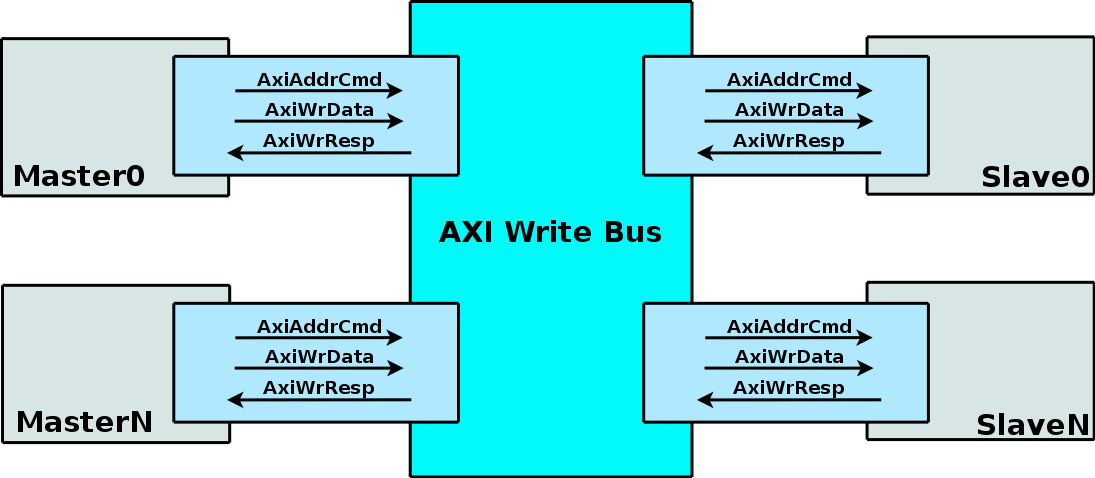
\includegraphics[height = 2 in]{AXIWrExample}
\caption{AXI Write Bus Example}
\label{AxiWrExample}
\end{center}
\end{figure}


The corresponding BSV AXI implementation is shown in figure
\ref{AxiWrTLM}.  TLM Write requests are received via the \te{TLMRecvIFC} 
interfaces of the master transactors. The request is then transmitted
via the \te{AxiWrMaster} interface out onto the AXI bus and on to the
appropriate slave transactor. The slave transactor receives the request via the
\te{AxiWrSlave} interface, translates the request back into a stream of 
TLM objects, and then transmits those objects via the \te{TLMSendIFC} 
interface. The TLM response from the write operation follows the 
same path in reverse.



\begin{figure}[ht]
\begin{center}
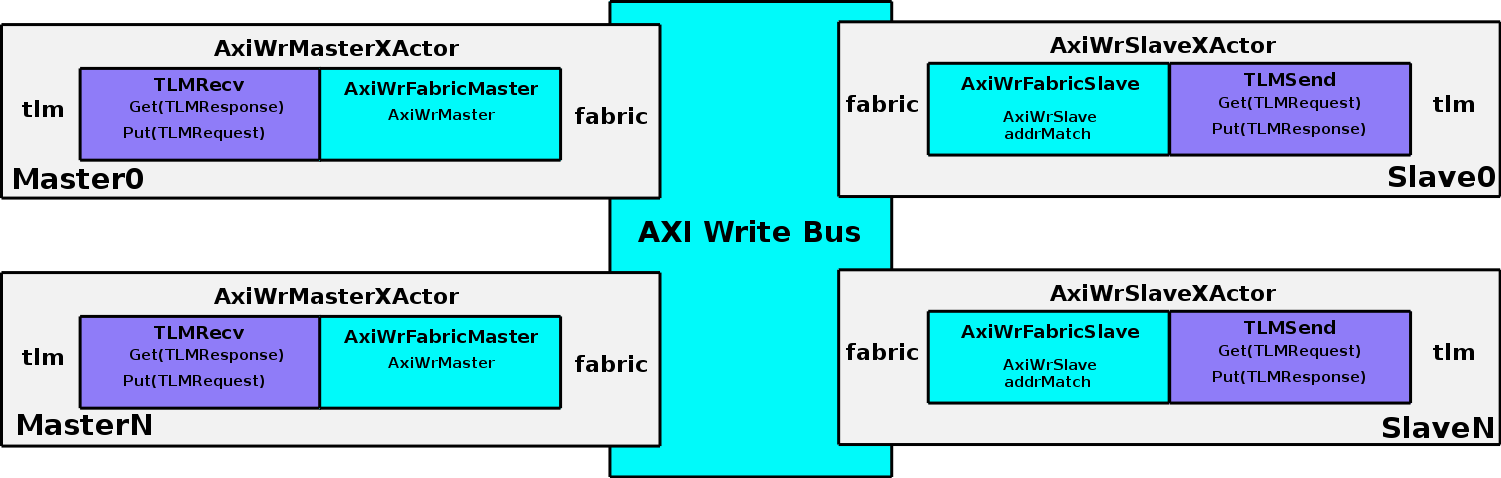
\includegraphics[width = 6 in]{AXIWrTLM}
\caption{BSV AXI Write Bus Implementation Using TLM Transactors}
\label{AxiWrTLM}
\end{center}
\end{figure}



{\bf Data Structures}
%\index{AxiAddrCmd@\te{AxiAddrCmd} (data structure)}
%\index{AxiId@\te{AxiId} (data type)}
%\index{AxiLen@\te{AxiLen} (data type)}
%\index{AxiSize@\te{AxiSize} (data type)}
%\index{AxiBurst@\te{AxiBurst} (data type)}
%\index{AxiLock@\te{AxiLock} (data type)}
%\index{AxiCache@\te{AxiCache} (data type)}
%\index{AxiProt\te{AxiProt} (data type)}
%\index{AxiAddr\te{AxiAddr} (data type)}

Inside the transactor modules, the AXI data is organized into the
following data structures: the address data is defined by
\te{AxiAddrCmd}, the read response is defined by \te{AxiRdResp}, the
write data is defined by \te{AxiWrData} and the write response is
defined by \te{AxiWrResp}.

\paragraph{\bf AxiAddrCmd} The AXI Address Bus is defined by a structure, \te{AxiAddrCmd}, the
components of which are described in the following table.

\begin{center}
\begin{tabular}{|p{1 in}|p{1.8in}|p{3.2 in}|}
\hline
\multicolumn{3}{|c|}{AxiAddrCmd} \\
\hline
\multicolumn{1}{|c|}{Member Name}&\multicolumn{1}{|c|}{DataType}&\multicolumn{1}{|c|}{Valid Values} \\
\hline
\hline
\te{id}&\te{AxiId\#(`TLM\_PRM)}&\te{Bit\#(id\_size)}\\
\hline
\te{len}&\te{AxiLen}&\te{Bit\#(4)}\\
\hline
\te{size}&\te{AxiSize}  &\te{Bit\#(3)}\\
\hline
\te{burst}&\te{AxiBurst}&FIXED, INCR, WRAP\\
\hline
\te{lock}&\te{AxiLock}&NORMAL, EXCLUSIVE, LOCKED\\
\hline
\te{cache}&\te{AxiCache}&\te{Bit\#(4)}\\
\hline
\te{prot}&\te{AxiProt}&\te{Bit\#(3)}\\
\hline
\te{addr}&\te{AxiAddr\#(`TLM\_PRM)}&\te{Bit\#(addr\_size)}\\
\hline
\end{tabular}
\end{center}

% \te{AxiDataEn}&\te{Bit\#(8)}& 1 bit per 8 bits of Axidata, for write
% enables\\
% \te{AxiOp}&&Read, Write\\

\begin{verbatim}
typedef struct {
                AxiId#(`TLM_PRM)   id;
                AxiLen               len;   
                AxiSize              size;
                AxiBurst             burst;   
                AxiLock              lock;   
                AxiCache             cache;   
                AxiProt              prot;   
                AxiAddr#(`TLM_PRM) addr;
                } AxiAddrCmd#(`TLM_PRM_DCL) deriving(Bits,Eq);
\end{verbatim}

\paragraph{\bf AxiRdResp} The AXI Read Bus is defined by the \te{AxiRdResp} structure, the
                components of which are described in the following
                table. 
%\index{AxiRdResp@\te{AxiRdResp} (data structure)}
%\index{AxiId@\te{AxiId} (data type)}
%\index{AxiData@\te{AxiData} (data type)}
%\index{AxiResp@\te{AxiResp} (data type)}


\begin{center}
\begin{tabular}{|p{1 in}|p{1.8in}|p{3.2 in}|}
\hline
\multicolumn{3}{|c|}{AxiRdResp} \\
\hline
\multicolumn{1}{|c|}{Member Name}&\multicolumn{1}{|c|}{DataType}&\multicolumn{1}{|c|}{Valid Values} \\
\hline
\hline
\te{id}&\te{AxiId\#(`TLM\_PRM)}&\te{Bit\#(id\_size)}\\
\hline
\te{data}&\te{AxiData\#(`TLM\_PRM)}&\te{Bit\#(data\_size)}\\
\hline
\te{resp}&\te{AxiResp}&OKAY, EXOKAY, SLVERR, DECERR\\
\hline
\te{last}&Bool&True, False\\
\hline
\end{tabular}
\end{center}

\begin{verbatim}
typedef struct {
                AxiId#(`TLM_PRM)   id;
                AxiData#(`TLM_PRM) data;
                AxiResp              resp;
                Bool                 last;
                } AxiRdResp#(`TLM_PRM_DCL) deriving(Bits,Eq);
\end{verbatim}


The AXI Write Bus is defined by  two structures, \te{AxiWrData} and
\te{AxiWrResp}.

%\index{AxiWrData@\te{AxiWrData} (data structure)}
%\index{AxiId@\te{AxiId} (data type)}
%\index{AxiData@\te{AxiData} (data type)}
%\index{AxiByteEn@\te{AxiByteEn} (data type)}


\paragraph{\bf AxiWrData} The components of \te{AxiWrData} are described in the following table.

\begin{center}
\begin{tabular}{|p{1 in}|p{1.8in}|p{3.2in}|}
\hline
\multicolumn{3}{|c|}{AxiWrData} \\
\hline
\multicolumn{1}{|c|}{Member Name}&\multicolumn{1}{|c|}{DataType}&\multicolumn{1}{|c|}{Valid Values} \\
\hline
\hline
\te{id}&\te{AxiId\#(`TLM\_PRM)}&\te{Bit\#(id\_size)}\\
\hline
\te{data}&\te{AxiData\#(`TLM\_PRM)}&\te{Bit\#(data\_size)}\\
\hline
\te{strb}&\te{AxiByteEn\#(`TLM\_PRM)}&\te{Bit\#(TDiv\#(data\_size, 8))}\\
\hline
\te{last}&Bool&True, False\\
\hline
\end{tabular}
\end{center}

\begin{verbatim}
typedef struct {
                AxiId#(`TLM_PRM)     id;
                AxiData#(`TLM_PRM)   data;
                AxiByteEn#(`TLM_PRM) strb;
                Bool                   last;
                } AxiWrData#(`TLM_PRM_DCL) deriving(Bits,Eq);
\end{verbatim}


\paragraph{\bf AxiWrResp} The components of \te{AxiWrResp}  are described in the following table.

%\index{AxiWrResp@\te{AxiWrResp} (data structure)}
%\index{AxiId@\te{AxiId} (data type)}
%\index{AxiResp@\te{AxiResp} (data type)}



\begin{center}
\begin{tabular}{|p{1 in}|p{1.8in}|p{3.2in}|}
\hline
\multicolumn{3}{|c|}{AxiWrResp} \\
\hline
\multicolumn{1}{|c|}{Member Name}&\multicolumn{1}{|c|}{DataType}&\multicolumn{1}{|c|}{Valid Values} \\
\hline
\hline
\te{id}&\te{AxiId\#(`TLM\_PRM)}&\te{Bit\#(id\_size)}\\
\hline
\te{resp}&\te{AxiResp}&OKAY, EXOKAY, SLVERR, DECERR\\
\hline
\end{tabular}
\end{center}

\begin{verbatim}
typedef struct {
                AxiId#(`TLM_PRM)   id;
                AxiResp              resp;
                } AxiWrResp#(`TLM_PRM_DCL) deriving(Bits,Eq);
\end{verbatim}


{\bf Bus Interfaces}
\label{sec-AXI-interfaces}

This section describes the AXI bus master and slave interfaces used by
the AXI transactor modules. Since the AXI protocol supports read and
write operations on separate buses, two flavors of each interface
exist, one for reads and one for writes.

%\index{AxiRdMaster@\te{AxiRdMaster} (interface)}
%\index{AxiWrMaster@\te{AxiWrMaster} (interface)}

\paragraph{\bf AxiRdMaster} The \te{AxiRdMaster} interface issues AXI 
read requests and receives AXI read responses. 

\begin{verbatim}
interface AxiRdMaster#(`TLM_PRM_DCL);
   // Address Outputs
   method AxiId#(`TLM_PRM)   arID;
   method AxiAddr#(`TLM_PRM) arADDR;
   method AxiLen               arLEN;
   method AxiSize              arSIZE;
   method AxiBurst             arBURST;
   method AxiLock              arLOCK;
   method AxiCache             arCACHE;
   method AxiProt              arPROT;
   method Bool                 arVALID;
      
   // Address Inputs
   method Action arREADY(Bool value);
      
   // Response Outputs
   method Bool                   rREADY;
      
   // Response Inputs
   method Action rID   (AxiId#(`TLM_PRM)   value);
   method Action rDATA (AxiData#(`TLM_PRM) value);
   method Action rRESP (AxiResp              value);
   method Action rLAST (Bool                 value);
   method Action rVALID(Bool                 value);
endinterface
\end{verbatim}

\paragraph{\bf AxiWrMaster} The \te{AxiWrMaster} interface issues AXI 
write requests and receives AXI write responses. 

\begin{verbatim}          
interface AxiWrMaster#(`TLM_PRM_DCL);
   // Address Outputs
   method AxiId#(`TLM_PRM)   awID;
   method AxiAddr#(`TLM_PRM) awADDR;
   method AxiLen               awLEN;
   method AxiSize              awSIZE;
   method AxiBurst             awBURST;
   method AxiLock              awLOCK;
   method AxiCache             awCACHE;
   method AxiProt              awPROT;
   method Bool                 awVALID;
      
   // Address Inputs
   method Action awREADY(Bool value);
      
   // Data Outputs
   method AxiId#(`TLM_PRM)     wID;
   method AxiData#(`TLM_PRM)   wDATA;
   method AxiByteEn#(`TLM_PRM) wSTRB;
   method Bool                   wLAST;
   method Bool                   wVALID;
      
   // Data Inputs
   method Action wREADY(Bool value);
      
   // Response Outputs
   method Bool                   bREADY;
      
   // Response Inputs
   method Action bID   (AxiId#(`TLM_PRM) value);
   method Action bRESP (AxiResp            value);
   method Action bVALID(Bool               value);
endinterface
\end{verbatim}

% \begin{figure}[ht]
% \begin{center}
% \includegraphics[height = 1.4 in]{AXISlave}
% \caption{BSV AXISlave Interface}
% \label{Axislave}
% \end{center}
% \end{figure}
%\index{AxiRdSlave@\te{AxiRdSlave} (interface)}
%\index{AxiWrSlave@\te{AxiWrSlave} (interface)}

\paragraph{\bf AxiRdSlave} The \te{AxiRdSlave} interface receives AXI 
read requests and returns AXI read responses. 

\begin{verbatim}
interface AxiRdSlave#(`TLM_PRM_DCL);
   // Address Inputs
   method Action arID   (AxiId#(`TLM_PRM)   value);
   method Action arADDR (AxiAddr#(`TLM_PRM) value);
   method Action arLEN  (AxiLen               value);
   method Action arSIZE (AxiSize              value);
   method Action arBURST(AxiBurst             value);
   method Action arLOCK (AxiLock              value);
   method Action arCACHE(AxiCache             value);
   method Action arPROT (AxiProt              value);   
   method Action arVALID(Bool                 value);
      
   // Address Outputs
   method Bool arREADY;
      
   // Response Inputs
   method Action rREADY(Bool value);
      
   // Response Outputs
   method AxiId#(`TLM_PRM)   rID;
   method AxiData#(`TLM_PRM) rDATA;
   method AxiResp              rRESP;
   method Bool                 rLAST;
   method Bool                 rVALID;
endinterface
\end{verbatim}

\paragraph{\bf AxiWrSlave} The \te{AxiWrSlave} interface receives AXI 
write requests and returns AXI write responses. 

\begin{verbatim}          
interface AxiWrSlave#(`TLM_PRM_DCL);
   // Address Inputs
   method Action awID   (AxiId#(`TLM_PRM)   value);
   method Action awADDR (AxiAddr#(`TLM_PRM) value);
   method Action awLEN  (AxiLen               value);
   method Action awSIZE (AxiSize              value);
   method Action awBURST(AxiBurst             value);
   method Action awLOCK (AxiLock              value);
   method Action awCACHE(AxiCache             value);
   method Action awPROT (AxiProt              value);   
   method Action awVALID(Bool                 value);
      
   // Address Outputs
   method Bool awREADY;
      
   // Data Inputs
   method Action wID   (AxiId#(`TLM_PRM)     value);
   method Action wDATA (AxiData#(`TLM_PRM)   value);
   method Action wSTRB (AxiByteEn#(`TLM_PRM) value);
   method Action wLAST (Bool                   value);
   method Action wVALID(Bool                   value);
      
   // Data Ouptuts
   method Bool wREADY;
      
   // Response Inputs
   method Action bREADY(Bool value);
      
   // Response Outputs
   method AxiId#(`TLM_PRM) bID;
   method AxiResp            bRESP;
   method Bool               bVALID;
endinterface
\end{verbatim}

The \te{AxiRdMaster} and \te{AxiRdSlave} interfaces as well as the
\te{AxiWrMaster} and \te{AxiWrSlave} interfaces are connectable.

\begin{verbatim}
instance Connectable#(AxiRdMaster#(`TLM_PRM), AxiRdSlave#(`TLM_PRM));

instance Connectable#(AxiWrMaster#(`TLM_PRM), AxiWrSlave#(`TLM_PRM));
\end{verbatim}

{\bf Fabric Interfaces}

When used in the context of a bus or switch, AXI transactor modules
must communicate with address decoding logic. As with the BSV
implementation of the AHB bus, bus fabric interfaces are provided
to support this communication. Unlike the AHB protocol however, with
the AXI bus protocol no explicit communication between the arbiter and
the master transactor modules is required. Thus the
\te{AxiRdFabricMaster} and \te{AxiWrFabricMaster} interfaces are simply 
wrappers around the bus interfaces themselves.

\begin{verbatim}
interface AxiRdFabricMaster#(`TLM_PRM_DCL);
   (* prefix = "" *)
   interface AxiRdMaster#(`TLM_PRM) bus;
endinterface
\end{verbatim}

\begin{verbatim}
interface AxiWrFabricMaster#(`TLM_PRM_DCL);
   (* prefix = "" *)
   interface AxiWrMaster#(`TLM_PRM) bus;
endinterface
\end{verbatim}

The \te{AxiRdFabricSlave} and \te{AxiWrFabricSlave} interfaces each
provide an \te{addrMatch} method which given an AXI address returns
an Boolean value indicating whether the given address maps to the
associated slave. By polling this method for each slave on the bus,
the decoding logic can determine the appropriate destination for each
bus transaction. 

\begin{verbatim}
interface AxiRdFabricSlave#(`TLM_PRM_DCL);
   (* prefix = "" *)
   interface AxiRdSlave#(`TLM_PRM) bus;
   method Bool addrMatch(AxiAddr#(`TLM_PRM) value);
endinterface
\end{verbatim}

\begin{verbatim}
interface AxiWrFabricSlave#(`TLM_PRM_DCL);
   (* prefix = "" *)
   interface AxiWrSlave#(`TLM_PRM) bus;
   method Bool addrMatch(AxiAddr#(`TLM_PRM) value);
endinterface
\end{verbatim}

{\bf Transactor Interfaces}
\label{Axi-transactors}
%\index{Transactors}

Each AXI transactor module provides AXI and TLM interfaces to
implement a translation between a stream of TLM operations and the AXI
bus protocol.  Each transactor has two subinterfaces: a subinterface
for the connection with the AXI bus and a subinterface to send and
receive TLM objects.  The AXI library package includes two master
transactor interfaces and two slave transactor interfaces; The
\te{AXIRdMasterXActor} and \te{AXIWrMasterXActor} interfaces for 
masters and the \te{AXIRdSlaveXActor} and \te{AXIWrSlaveXActor}
interfaces for slaves.  Since the AXI protocol supports read and write
transaction on separate buses, two transactor implementations are
required for masters and two implementations for slaves.  The AXI
subinterface definitions can be found in section
\ref{sec-AXI-interfaces}.


\paragraph{\bf AxiRdMasterXActorIFC} The \te{AxiRdMasterXActorIFC} has two subinterfaces: 
an \te{AxiRdFabricMaster} subinterface and a \te{TLMRecvIFC}
subinterface.  The associated transactor converts TLM read requests
into the AXI protocol, and converts the AXI response back into TLM.

%\index{AxiRdMasterXActorIFC@\te{AxiRdMasterXActorIFC} (interface)}        

\begin{verbatim}
interface AxiRdMasterXActorIFC#(`TLM_RR_DCL, `TLM_PRM_DCL);
   interface TLMRecvIFC#(`TLM_RR)        tlm;
   (* prefix = "" *)
   interface AxiRdFabricMaster#(`TLM_PRM) fabric;
endinterface
\end{verbatim}

\paragraph{\bf AxiWrMasterXActorIFC} The \te{AxiWrMasterXActorIFC} has two subinterfaces: 
an \te{AxiWrFabricMaster} subinterface and a \te{TLMRecvIFC}
subinterface.  The associated transactor converts TLM write requests
into the AXI protocol, and converts the AXI response back into TLM.

%\index{AxiWrMasterXActorIFC@\te{AxiWrMasterXActorIFC} (interface)}        

\begin{verbatim}
interface AxiWrMasterXActorIFC#(`TLM_RR_DCL, `TLM_PRM_DCL);
   interface TLMRecvIFC#(`TLM_RR)        tlm;
   (* prefix = "" *)
   interface AxiWrFabricMaster#(`TLM_PRM) fabric;
endinterface
\end{verbatim}


\begin{figure}[ht]
\begin{center}
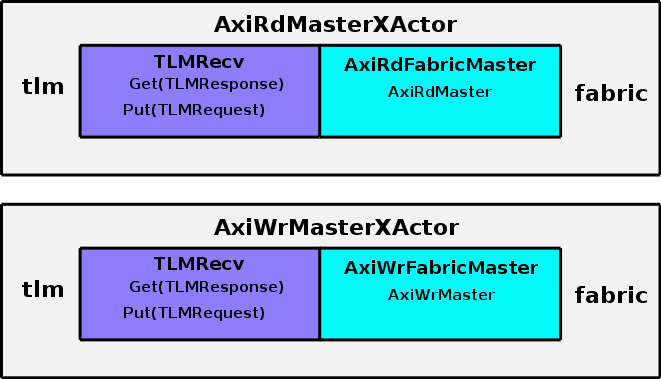
\includegraphics[height = 2 in]{AXIMasterXActor}
\caption{AXIMasterXActor Interfaces (Read and Write Versions)}
\label{AxiMasterXActor}
\end{center}
\end{figure}


\paragraph{\bf AxiRdSlaveXActorIFC} The \te{AxiRdSlaveXActorIFC} has two subinterfaces:
an \te{AxiRdFabricSlave} subinterface and a \te{TLMSendIFC}
subinterface. The associated transactor converts an AXI read request
into TLM and the TLM response back into the AXI protocol.

%\index{AxiRdSlaveXActorIFC@\te{AxiRdSlaveXActorIFC} (interface)}        

\begin{verbatim}
interface AxiRdSlaveXActorIFC#(`TLM_RR_DCL, `TLM_PRM_DCL);
   interface TLMSendIFC#(`TLM_RR)       tlm;
   (* prefix = "" *)
   interface AxiRdFabricSlave#(`TLM_PRM) fabric;
endinterface
\end{verbatim}

\paragraph{\bf AxiWrSlaveXActorIFC} The \te{AxiWrSlaveXActorIFC} has two subinterfaces:
an \te{AxiWrFabricSlave} subinterface and a \te{TLMSendIFC}
subinterface. The associated transactor converts an AXI write request
into TLM and the TLM response back into the AXI protocol.

%\index{AxiWrSlaveXActorIFC@\te{AxiWrSlaveXActorIFC} (interface)}        

\begin{verbatim}
interface AxiWrSlaveXActorIFC#(`TLM_RR_DCL, `TLM_PRM_DCL);
   interface TLMSendIFC#(`TLM_RR)       tlm;
   (* prefix = "" *)
   interface AxiWrFabricSlave#(`TLM_PRM) fabric;
endinterface
\end{verbatim}

\begin{figure}[ht]
\begin{center}
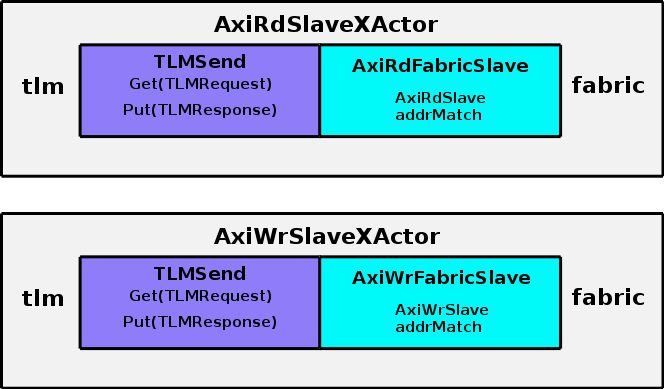
\includegraphics[height = 2 in]{AXISlaveXActor}
\caption{AXISlaveXActor Interfaces (Read and Write Versions)}
\label{AxiSlaveXActor}
\end{center}
\end{figure}

{\bf Modules}

The following constructors are used to create AXI transactor modules.  Versions
with associated synthesis boundaries are also available. These
versions are called \te{mkAxiRdMasterStd}, \te{mkAxiWrMasterStd}, \te{mkAxiRdSlaveStd}, 
and \te{mkAxiWrSlaveStd}. The specific TLM parameter values for these 
synthesized versions are as specified by the preprocessor macro \te{TLM\_STD\_TYPES}.

%\index{mkAxiRdMaster@\te{mkAxiRdMaster} (module)}
%\index[function]{AXI!mkAxiRdMaster}

\begin{center}
\begin{tabular}{|p{1 in}|p{5.2 in}|}
\hline 
&\\
\te{mkAxiRdMaster}&Creates an AXI master read transactor module. Provides an \te{AxiRdMasterXActorIFC} interface.  \\
&\\
\cline{2-2}
&\begin{libverbatim}
module mkAxiRdMaster (AxiRdMasterXActorIFC#(`TLM_XTR))
   provisos(Bits#(req_t, s0), 
            Bits#(resp_t, s1),
            TLMRequestTC#(req_t, `TLM_PRM),
            TLMResponseTC#(resp_t, `TLM_PRM),
            DefaultValue#(cstm_type),
            AxiConvert#(AxiProt, cstm_type)
            AxiConvert#(AxiCache, cstm_type),
            AxiConvert#(AxiLock, cstm_type));
\end{libverbatim}
\\
\hline
\end{tabular}
\end{center}

%\index{mkAxiWrMaster@\te{mkAxiWrMaster} (module)}
%\index[function]{AXI!mkAxiWrMaster}


\begin{center}
\begin{tabular}{|p{1 in}|p{5.2 in}|}
\hline 
&\\
\te{mkAxiWrMaster}&Creates an AXI master write transactor module. Provides an \te{AxiWrMasterXActorIFC} interface.  \\
&\\
\cline{2-2}
&\begin{libverbatim}
module mkAxiWrMaster (AxiWrMasterXActorIFC#(`TLM_XTR))
   provisos(Bits#(req_t, s0), 
            Bits#(resp_t, s1),
            TLMRequestTC#(req_t, `TLM_PRM),
            TLMResponseTC#(resp_t, `TLM_PRM),
            DefaultValue#(cstm_type),
            Bits#(cstm_type, s2),
            AxiConvert#(AxiProt, cstm_type)
            AxiConvert#(AxiCache, cstm_type),
            AxiConvert#(AxiLock, cstm_type));
\end{libverbatim}
\\
\hline
\end{tabular}
\end{center}

%\index{mkAxiRdSlave@\te{mkAxiRdSlave} (module)}
%\index[function]{AXI!mkAxiRdSlave}

\begin{center}
\begin{tabular}{|p{1 in}|p{5.2 in}|}
\hline 
&\\
\te{mkAxiRdSlave}&Creates an AXI slave read transactor module. Provides an \te{AxiRdSlaveXActorIFC} interface.  \\
&\\
\cline{2-2}
&\begin{libverbatim}
module mkAxiRdSlave#(Integer max_flight, 
                     function Bool addr_match(AxiAddr#(`TLM_PRM) addr)) 
	            (AxiRdSlaveXActorIFC#(`TLM_XTR))
   provisos (TLMRequestTC#(req_t, `TLM_PRM),
             TLMResponseTC#(resp_t, `TLM_PRM),
             Bits#(req_t, s0),
             Bits#(resp_t, s1),
             Bits#(cstm_type, s2),
             AxiConvert#(AxiCustom, cstm_type));
\end{libverbatim}
\\
\hline
\end{tabular}
\end{center}

%\index{mkAxiWrSlave@\te{mkAxiWrSlave} (module)}
%\index[function]{AXI!mkAxiWrSlave}

\begin{center}
\begin{tabular}{|p{1 in}|p{5.2 in}|}
\hline 
&\\
\te{mkAxiWrSlave}&Creates an AXI slave write transactor module. Provides an \te{AxiWrSlaveXActorIFC} interface.  \\
&\\
\cline{2-2}
&\begin{libverbatim}
module mkAxiWrSlave#(Integer max_flight, 
                     function Bool addr_match(AxiAddr#(`TLM_PRM) addr)) 
		    (AxiWrSlaveXActorIFC#(`TLM_XTR))
   provisos(TLMRequestTC#(req_t, `TLM_PRM),
            TLMResponseTC#(resp_t, `TLM_PRM),
            Bits#(req_t, s0),
            Bits#(resp_t, s1),
            Bits#(cstm_type, s2),
            AxiConvert#(AxiCustom, cstm_type));
\end{libverbatim}
\\
\hline
\end{tabular}
\end{center}

The following two module constructors are each used to create an AXI
bus fabric. \te{mkAxiRdBus} is used to create a read bus while
\te{mkAxiWrBus} is used to create a write bus.


%\index{@\te{mkAxiRdBus} (module)}
%\index[function]{AXI!mkAxiRdBus}

\begin{center}
\begin{tabular}{|p{1 in}|p{5.2 in}|}
\hline 
&\\
\te{mkAxiRdBus}&Given a vector of \te{AxiRdFabricMaster} interfaces and a vector 
of \te{AxiRdFabricSlave} interfaces, \te{mkAxiRdBus} creates an AXI read bus. \\
&\\
\cline{2-2}
&\begin{libverbatim}
module mkAxiRdBus#(Vector#(master_count, 
                           AxiRdFabricMaster#(`TLM_PRM)) masters, 
                   Vector#(slave_count,  
                           AxiRdFabricSlave#(`TLM_PRM))slaves) (Empty)
   provisos(Log#(master_count, size_m), 
            Add#(slv_count, 1, slave_count),
            Log#(slave_count, size_s),
            Add#(ignore0, size_m, id_size),
            Add#(ignore1, size_s, id_size));
\end{libverbatim}
\\
\hline
\end{tabular}
\end{center}


%\index{@\te{mkAxiWrBus} (module)}
%\index[function]{AXI!mkAxiWrBus}

\begin{center}
\begin{tabular}{|p{1 in}|p{5.2 in}|}
\hline 
&\\
\te{mkAxiWrBus}&Given a vector of \te{AxiWrFabricMaster} interfaces and a vector 
of \te{AxiWrFabricSlave} interfaces, \te{mkAxiWrBus} creates an AXI write bus. \\
&\\
\cline{2-2}
&\begin{libverbatim}
module mkAxiWrBus#(Vector#(master_count, 
                           AxiWrMaster#(`TLM_PRM)) masters, 
                   Vector#(slave_count,  
                           AxiWrSlave#(`TLM_PRM)) slaves) (Empty)
   provisos(Log#(master_count, size_m), 
            Add#(slv_count, 1, slave_count),
            Log#(slave_count, size_s),
            Add#(ignore0, size_m, id_size),
            Add#(ignore1, size_s, id_size));
\end{libverbatim}
\\
\hline
\end{tabular}
\end{center}

The following module is used to add probe signals for each of the AXI
bus signals. This facilitates debugging and waveform viewing of the created bus fabric.

%\index{@\te{mkAxiMonitor} (module)}
%\index[function]{AXI!mkAxiMonitor}

\begin{center}
\begin{tabular}{|p{1 in}|p{5.2 in}|}
\hline 
&\\
\te{mkAxiMonitor}&Adds a probe module for each of the AXI bus signals.
The \te{include\_pc} value indicates
whether or not the monitor module should include an instantiation of
an AXI protocol checker module (available from ARM).  If the protocol
checker is not available, the value of \te{include\_pc} should be set to False.  \\
&\\
\cline{2-2}
&\begin{libverbatim}
module mkAxiMonitor#(Bool include_pc,
                     AxiWrMaster#(`TLM_PRM) master_wr,
                     AxiWrSlave#(`TLM_PRM)  slave_wr,
                     AxiRdMaster#(`TLM_PRM) master_rd,
                     AxiRdSlave#(`TLM_PRM)  slave_rd) 
                     (AxiMonitor#(`TLM_PRM));
\end{libverbatim}
\\
\hline
\end{tabular}
\end{center}

{\bf Functions}

The following functions convert from TLM to AXI

%\index{getAxiAddrCmd@\te{getAxiAddrCmd} (function)}
%\index[function]{AXI!getAxiAddrCmd}

\begin{center}
\begin{tabular}{|p{1.2 in}|p{5 in}|}
\hline 
&\\
\te{getAxiAddrCmd}&Returns an \te{AxiAddrCmd} from a TLM \te{RquestDescriptor}   \\
&\\
\cline{2-2}
&\begin{libverbatim}
function AxiAddrCmd#(`TLM_PRM) getAxiAddrCmd (
                      RequestDescriptor#(`TLM_PRM) tlm_descriptor)
   provisos(AxiConvert#(AxiProt, cstm_type),
            AxiConvert#(AxiCache, cstm_type),
            AxiConvert#(AxiLock, cstm_type) );
\end{libverbatim}
\\
\hline
\end{tabular}
\end{center}

%\index{getFirstAxiWrData@\te{getFirstAxiWrData} (function)}
%\index[function]{AXI!getFirstAxiWrData}

\begin{center}
\begin{tabular}{|p{1.2in}|p{5 in}|}
\hline 
&\\
\te{getFirstAxiWrData}& Returns the \te{AxiWrData} from the TLM 
\te{RequestDesriptor}  \\
&\\
\cline{2-2}
&\begin{libverbatim}
function AxiWrData#(`TLM_PRM) getFirstAxiWrData (
                     RequestDescriptor#(`TLM_PRM) tlm_descriptor);
\end{libverbatim}
\\
\hline
\end{tabular}
\end{center}

%\index{getAxiByteEn@\te{getAxiByteEn} (function)}
%\index[function]{AXI!getAxiByteEn}

\begin{center}
\begin{tabular}{|p{1.2 in}|p{5 in}|}
\hline 
&\\
\te{getAxiByteEn}& Returns the \te{AxiByteEn} from the TLM \te{RequestDesriptor}  \\
&\\
\cline{2-2}
&\begin{libverbatim}
function AxiByteEn#(`TLM_PRM) getAxiByteEn (
                     RequestDescriptor#(`TLM_PRM) tlm_descriptor);
\end{libverbatim}
\\
\hline
\end{tabular}
\end{center}

%\index{getAxiLen@\te{getAxiLen} (function)}
%\index[function]{AXI!getAxiLen}

\begin{center}
\begin{tabular}{|p{1.2 in}|p{5 in}|}
\hline 
&\\
\te{getAxiLen}&Returns the \te{AxiLen} from the TLM \te{burst\_length}   \\
&\\
\cline{2-2}
&\begin{libverbatim}
function AxiLen getAxiLen(TLMUInt#(`TLM_PRM) burst_length);
\end{libverbatim}
\\
\hline
\end{tabular}
\end{center}

%\index{getAxiSize@\te{getAxiSize} (function)}
%\index[function]{AXI!getAxiSize}

\begin{center}
\begin{tabular}{|p{1.2 in}|p{5 in}|}
\hline 
&\\
\te{getAxiSize}&Returns the \te{AxiSize} from the TLM \te{incr}   \\
&\\
\cline{2-2}
&\begin{libverbatim}
function AxiSize getAxiSize(TLMBurstSize#(`TLM_PRM) incr);
\end{libverbatim}
\\
\hline
\end{tabular}
\end{center}

%\index{getAxiSize@\te{getAxiSize} (function)}
%\index[function]{AXI!getAxiSize}

\begin{center}
\begin{tabular}{|p{1.2 in}|p{5 in}|}
\hline 
&\\
\te{getAxiSize}&Returns the \te{AxiSize} from the TLM \te{incr}   \\
&\\
\cline{2-2}
&\begin{libverbatim}
function AxiSize getAxiSize(TLMBurstSize#(`TLM_PRM) incr);
\end{libverbatim}
\\
\hline
\end{tabular}
\end{center}


%\index{getAxiBurst@\te{getAxiBurst} (function)}
%\index[function]{AXI!getAxiBurst}

\begin{center}
\begin{tabular}{|p{1.2 in}|p{5 in}|}
\hline 
&\\
\te{getAxiBurst}& Returns the \te{AxiBurst} from the TLM \te{burst\_mode}  \\
&\\
\cline{2-2}
&\begin{libverbatim}
function AxiBurst getAxiBurst(TLMBurstMode burst_mode);
\end{libverbatim}
\\
\hline
\end{tabular}
\end{center}

%\index{getAxiId@\te{getAxiId} (function)}
%\index[function]{AXI!getAxiId}

\begin{center}
\begin{tabular}{|p{1.2 in}|p{5 in}|}
\hline 
&\\
\te{getAxiId}&Returns the \te{AxiId} from the TLM \te{transaction\_id}   \\
&\\
\cline{2-2}
&\begin{libverbatim}
function AxiId#(`TLM_PRM) getAxiId(TLMId#(`TLM_PRM) transaction_id);
\end{libverbatim}
\\
\hline
\end{tabular}
\end{center}

The following functions convert from Axi to TLM

%\index{fromAxiAddrCmd@\te{fromAxiAddrCmd} (function)}
%\index[function]{AXI!fromAxiAddrCmd}

\begin{center}
\begin{tabular}{|p{1.2 in}|p{5 in}|}
\hline 
&\\
\te{fromAxiAddrCmd}& Returns the TLM \te{RequestDescriptor} from the
AXI \te{addr\_cmd}  \\
&\\
\cline{2-2}
&\begin{libverbatim}
function RequestDescriptor#(`TLM_PRM) fromAxiAddrCmd (
              AxiAddrCmd#(`TLM_PRM) addr_cmd)
   provisos(Bits#(RequestDescriptor#(`TLM_PRM), s0),
            AxiConvert#(AxiCustom, cstm_type));
\end{libverbatim}
\\
\hline
\end{tabular}
\end{center}

%\index{fromAxiLen@\te{fromAxiLen} (function)}
%\index[function]{AXI!fromAxiLen}

\begin{center}
\begin{tabular}{|p{1.2 in}|p{5 in}|}
\hline 
&\\
\te{fromAxiLen}& Returns the TLM \te{burst\_length} from the AXI \te{len}  \\
&\\
\cline{2-2}
&\begin{libverbatim}
function TLMUInt#(`TLM_PRM) fromAxiLen(AxiLen len);
\end{libverbatim}
\\
\hline
\end{tabular}
\end{center}


%\index{fromAxiBurst@\te{fromAxiBurst} (function)}
%\index[function]{AXI!fromAxiBurst}

\begin{center}
\begin{tabular}{|p{1.2 in}|p{5 in}|}
\hline 
&\\
\te{fromAxiBurst}& Returns the TLM \te{burst\_mode} from the AXI \te{burst}  \\
&\\
\cline{2-2}
&\begin{libverbatim}
function TLMBurstMode fromAxiBurst(AxiBurst burst);
\end{libverbatim}
\\
\hline
\end{tabular}
\end{center}


%\index{fromAxiSize@\te{fromAxiSize} (function)}
%\index[function]{AXI!fromAxiSize}

\begin{center}
\begin{tabular}{|p{1.2 in}|p{5 in}|}
\hline 
&\\
\te{fromAxiSize}&  Returns the TLM \te{burst\_size} from the AXI \te{size} \\
&\\
\cline{2-2}
&\begin{libverbatim}
function TLMBurstSize#(`TLM_PRM) fromAxiSize(AxiSize size);
\end{libverbatim}
\\
\hline
\end{tabular}
\end{center}

%\index{fromAxiId@\te{fromAxiId} (function)}
%\index[function]{AXI!fromAxiId}

\begin{center}
\begin{tabular}{|p{1.2 in}|p{5 in}|}
\hline 
&\\
\te{fromAxiId}&Returns a TLM \te{id} from the AXI \te{id}   \\
&\\
\cline{2-2}
&\begin{libverbatim}
function TLMId#(`TLM_PRM) fromAxiId(AxiId#(`TLM_PRM) id);
\end{libverbatim}
\\
\hline
\end{tabular}
\end{center}

%\index{fromAxiResp@\te{fromAxiResp} (function)}
%\index[function]{AXI!fromAxiResp}

\begin{center}
\begin{tabular}{|p{1.2 in}|p{5 in}|}
\hline 
&\\
\te{fromAxiResp}&Returns the TLM \te{status}  from the AXI \te{resp}   \\
&\\
\cline{2-2}
&\begin{libverbatim}
function TLMStatus fromAxiResp(AxiResp resp);
\end{libverbatim}
\\
\hline
\end{tabular}
\end{center}

\end{document}
